\section{Proposed Architecture} \label{arch}

We now discuss the main components necessary to realize a practical Tor route assignment system.

\subsection{Overview}
We propose a system that measures the end-to-end bandwidth contributed to the Tor network to incentivise the addition of nodes to the Tor network.

The system measures the bandwidth contributed by each relay in the Tor network and rewards them with a 'TorCoin'. A Torcoin is an AltCoin that uses a bandwidth-intensive protocol as its proof-of-work. Thus, to produce a TorCoin, a relay must have transmitted a certain amount of Tor traffic.

To reduce the system's vulnerability to attackers and possible reduction of anonymity, we also utilize the TorPaths system to randomly assign relays to clients.

These TorCoins can then be traded at an exchange for other AltCoins or other goods. This forms the basis of our incentivization scheme. This is different from systems that propose differentiated service\cite{dovrolis1999case, dovrolis2002proportional}, since we do not propose to make the clients pay for access to the network. The coins are a byproduct of the usage of the system.

\subsection{TorPaths}
The TorPaths system adheres to the following constraints:
\begin{itemize}
  \item No client in the group can generate its own route.
  \item Every resulting route has a unique public key ('Route signature').
  \item No client in the group can know the route assigned to another client in the group.
  \item Any interested party can verify that a given public key represents a route assigned to a client in a group.
\end{itemize}

\subsubsection{Setup}
The Tor Assigning Servers will create the consensus groups using the temporal locality of the clients connecting to them, but also ensure that there is geographical and other diversity in a group. This is to ensure that adversaries cannot deterministically place themselves in a single consensus group by connecting at the same time.

A consensus group consists of the first n = 1000 clients that have connected to the Assigning Servers. In practice, we expect the number n to be modulated so that groups are being created every 10 seconds or so. Consensus group diversity is implemented by ensuring that a group consists of a majority of the Assigning Servers. Thus, if there are 10 Assigning Servers in the entire network, a group must consist of atleast 6 of them. The clients are indexed by the order of their joining the group.

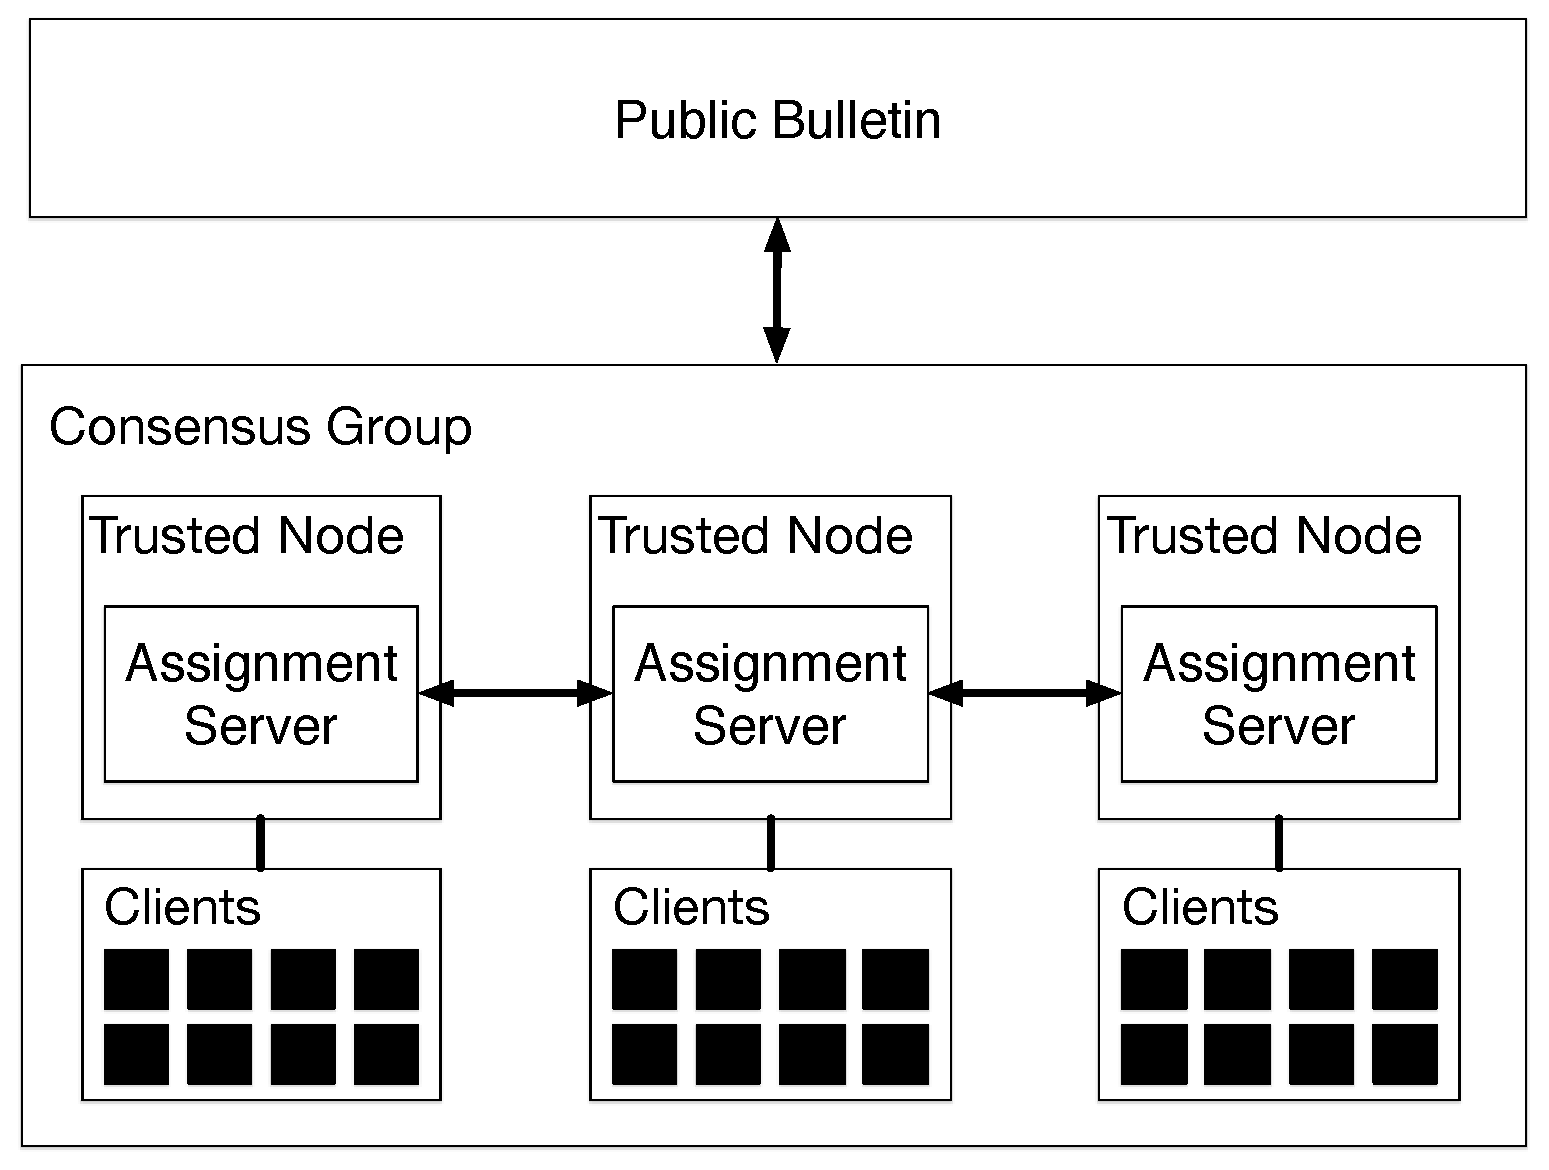
\includegraphics[scale=0.3]{torpath_grouping.pdf}

\subsubsection{Route Assignment using Neff shuffles}
Once all the clients have filled up the group, the Assigning Servers in the consensus group initiate the process of route assignment.

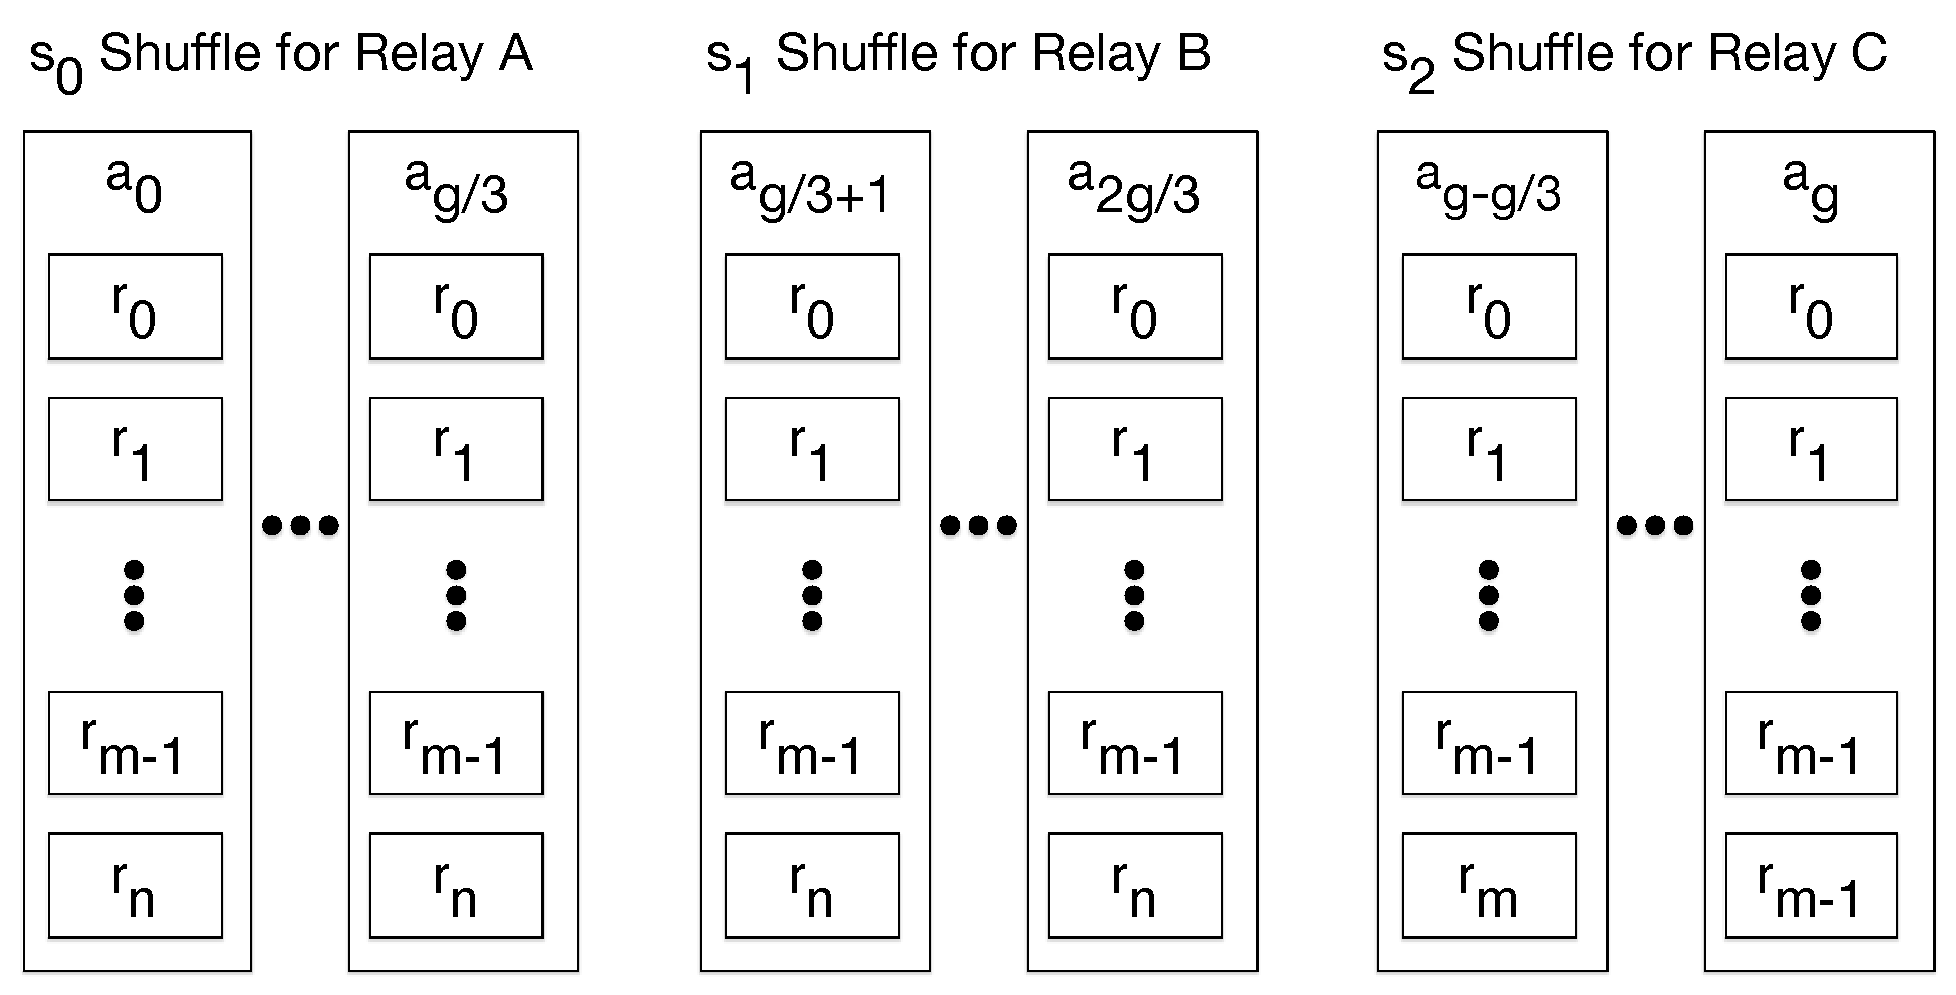
\includegraphics[scale=0.3]{torpath_shufflesets.pdf}

\begin{enumerate}
  \item The Assigning servers in the group are randomly divided into three 'Shuffle Sets'.
  \item Each set of Assigning servers uses a unique Neff shuffle to create shuffled lists of entry, middle and exit relays. The ith client in the consensus group is thus matched up with the ith entry, middle and exit relay to form a 'route'.
  \item The servers then create a route-signature for each route based on some property CLARIFY of each participant (client and three relays). One of the three server groups is also assigned to be the Route signature group. This group collects all the route signature keys.
  \item Each route-signature is then input into a cryptographic accumulator so that anyone can verify if a route belonged to a group. This accumulator is published in a publicly available log along with the timestamp of the group creation.
\end{enumerate}

Each server then sends each client in the group one piece of data. Eg: The servers that assigned the entry relays send each client its own entry relay. Similarly, the middle and exit relays and the route signatures are also communicated in the same way. Thus, each client knows its own [Entry, Middle, Exit relay, Route Signature] 
For each relay, the servers send an Access Control List. This is a list of all the relays and clients that the relay should accept connections from, as well as the route signatures for each.

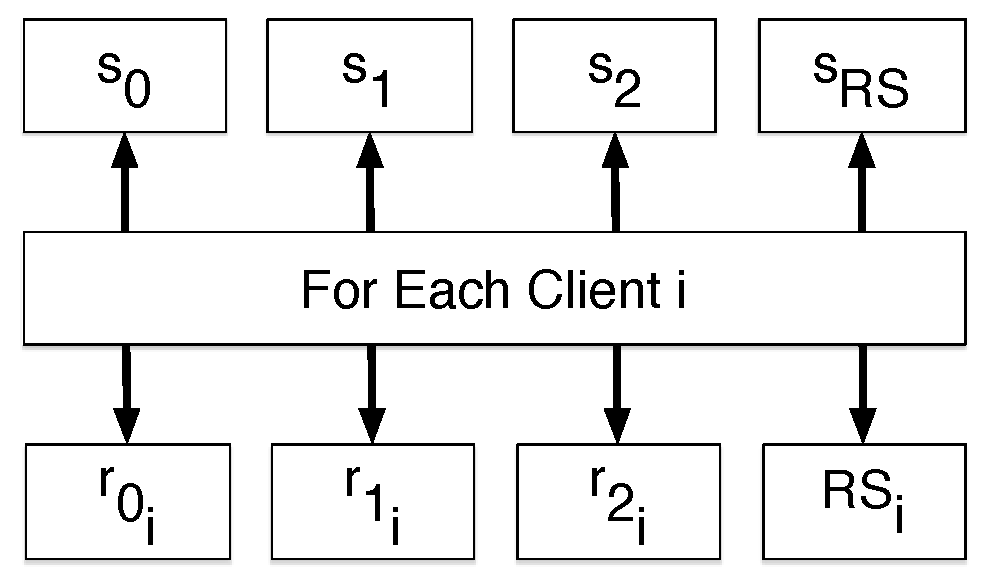
\includegraphics[scale=0.5]{torpath_result.pdf}

In this way, no single server is aware of any client's entire path through the network, preserving their anonymity. Since each point in the path is confirmed by atleast two servers, it is also robust to rogue servers.

Once these paths are formed, the client can communicate using the existing Tor protocol. 

\subsubsection{Proof of Bandwidth - Onion Hashing}
Once the routes are setup, we can prove end-to-end bandwidth transfer through the following protocol:
Every m Tor packets, the client sends an extra packet ('the Torcoin packet') containing an hash attempt likely to generate a TorCoin. Relay A gets it, generates a temporary private key Ka (generated using the route shared key) and hashes the received packet and this key. It then forwards it to B, which does the same thing, with its own private temporary key Kb. Similarly on to C. C can now add its own Kc, and if it generates a hash with a given number of zeros, it can claim to have found a TorCoin.
\begin{verbatim}
Client sends to A: T0 (its hash attempt)
A sends to B     : Hash(T0 + K1) = Ta # K1 is A's temporary private key.
B sends to C     : Hash(Ta + K2) = Tb # K2 is B’s temporary private key.
C computes       : Hash(Tb + K3) = Tc # K3 is C’s temporary private key.
C sends to B     : (Tc, K3) to verify.
B sends to A     : (Tc, K3, Tb, K2) to verify.
A sends to client: (Tc, K3, Tb, K2, Ta, K1) to verify.
\end{verbatim}
Once the client has verified the hash, we can confirm that the data has made a 
round trip through the route. This completes the proof of bandwidth.

\subsubsection{TorCoin}
We can then implement an AltCoin based on the proof-of-work in the following manner:
\begin{verbatim}
If (Tc = '000...')
  If the client succesfully verifies the hash
    It adds the coin to the blockchain with the following information:
    1. Timestamp of group.
    2. Client’s public key.
    3. Route Shared key (Lets any other group member verify that the route is 
       genuine. See accumulator.)
    4. TorCoin Hash.
    It then gives 1/3rd of the coin to each of the relays in the route. (If the 
    client is rogue, can we identify and kick the client off?)
\end{verbatim}
This information in the blockchain will enable any interested party to verify if the route came from a legitimate group formed by the directory servers. This can be done by taking the route signature and comparing it with the publicly available accumulators. 

The properties of the Altcoin will then take over, with clients building on the blockchain with more and more TorCoins that they mine through this process.

\subsection{Securty Considerations}
The TorPaths algorithm ensures that the Torcoin system robust to attackers. Due to the random group selection system, it is hard for attackers to deterministically place themselves in a group. To make the system even more secure, the servers can randomize group assignment instead of just taking temporal locality to be the criterion.

In addition, because the attacker needs to control all four components of a route to mint a TorCoin fraudulently, even if the adversaries control up to half the network, there is a probability of only 1/16 that an adversary client gets a path of three colluding relays. In practice, gaining control of half of the entire Tor client and relay network is practically impossible. 

A separate rate-limiting mechanism can be deployed to detect dishonest relays and remove them from the the path selection procedure. An independent verification authority, such as one based on Eigenspeed, could be used to detect these discrepancies.

The random grouping of clients, as well as the decentralized Neff shuffles ensure that all the clients are in the same anonymity set - similar to the current Tor implementation. It is not possible to partition the anonymity set because no part of the system, other than the client itself, is aware of the entire path of any client.

\subsection{Drawbacks}
The TorPath network is not backwards compatible with the existing Tor network, due to the fundamental differences of route assignment and access control, which are missing in Tor, but are necessary for the TorPath and TorCoin schemes to work.

However, our scheme does not preclude a given physical relay or server from running both services at the same time. They will, of course, only get paid for the TorCoin traffic. In time, we expect that a majority of the current Tor relay operators will switch over to the TorPath network, since TorPath has the same security guarantees as Tor provides, while also recompensing the relay operators for their costs.

While backwards-compatibility with Tor is a desired feature, a client's freedom to choose its own path is fundamentally opposed to the TorPath system.